
\subsection{Allocation View}\label{sec:storeAllocView}
Figure \ref{fig:deploymentDiagram} uses a UML deployment diagram as a visual representation of the physical architecture of the system as part of the allocation view.
The diagram also shows some of the important software components that are deployed onto parts of the physical architecture.
For simplicity, details such as load balancing and failover are not shown in this example.

\begin{figure}[h!]
    \centering
    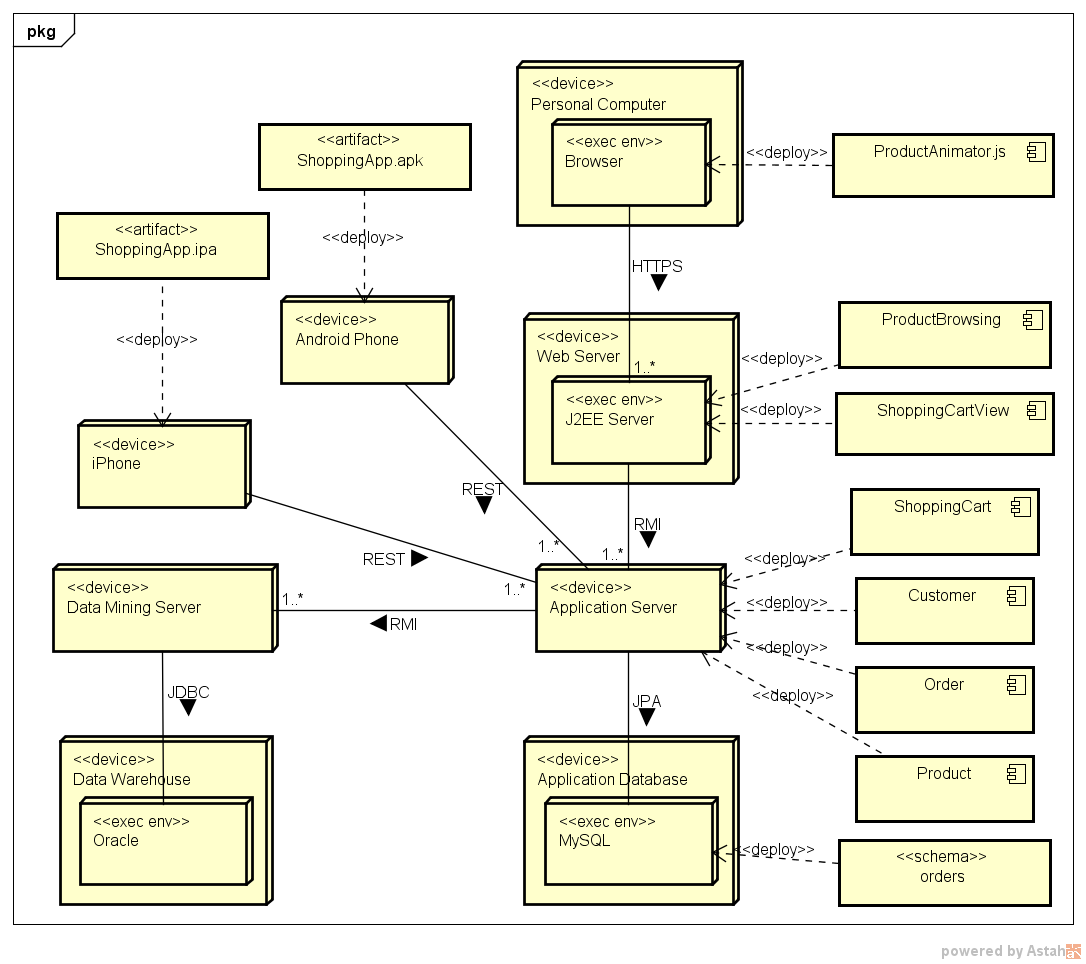
\includegraphics[trim=38 38 23 44,clip,width=0.95\textwidth]{images/uml/deployment_diagram.png}
    \caption{Example physical architecture for the Sahara eCommerce system.}
    \label{fig:deploymentDiagram}
\end{figure}

There are both web and mobile applications that customers use to shop at the store.
A J2EE server (e.g. \link{TomEE}{https://tomee.apache.org/}), running on a web server hardware platform,
handles browser requests from customers, using the HTTPS protocol over the Internet.
A JavaScript module called \texttt{ProductAnimator} is downloaded to the customer's browser to allow them to see interactive 3d views of products.
The \texttt{ProductBrowsing} and \texttt{ShoppingCartView} components run on the J2EE server, providing those aspects of the user interaction.
The J2EE server uses RMI\footnote{Remote Method Invocation} over a network connection to an application server.

The application server provides the shared logic of the on-line store.
This supports implementing the functional requirement that a customer can start shopping on one device and continue on another.
Running the applicaiton server on its own device allows easier scalability of the system.
The application server could be replicated on multiple devices to handle requests from different sources, without duplicating unneeded web or database logic.
Examples of components that would run on the application server are \texttt{Customer}, \texttt{ShoppingCart}, \texttt{Order} and \texttt{Product}.

The application server uses JPA\footnote{Java Persistence API} over a network connection to communicate with the application data\-base running on a separate server.
The \texttt{orders} schema is an example of one of the tables that would be created in the application database.
The application server also uses RMI over a network connection to communicate with a data mining server.

The data mining server uses JDBC\footnote{Java DataBase Connectivity} over a network connection to a server running the data warehouse.
The mobile applications run on their respective phone environments and use REST API calls over the Internet to interact with application server.

\textbf{Note}, for web applications the customer's computer and browser would only be shown in the deployment diagram
if the software system downloads application logic that executes in the browser (e.g. JavaScript).
In this example the \texttt{ProductAnimator.js} module is an important part of the application's functional requirements.

\subsubsection{Deployment Diagram Notation}\label{sec:deploymentNotation}
In the diagram, cube icons represent \emph{nodes}. Nodes are computational resources that can execute software artifacts.
Nodes may be \guillemotleft device\guillemotright's, representing hardware.
They may also be \guillemotleft executionEnvironment\guillemotright's, representing software that provides an environment in which other software artifacts can be executed.
(The keyword has been shortened to \guillemotleft exec env\guillemotright~in this example.)
Execution environments need to be allocated to devices.
In figure \ref{fig:deploymentDiagram}, \texttt{Browser} and \texttt{J2EE Server} are software environments running,
respectively, on the hardware devices \texttt{Personal Computer} and \texttt{Web Server}.

The solid lines between nodes are \emph{associations}, which represent communication paths.
A communication path can represent a \emph{physical connection} or \emph{protocol}.
Formally, a stereotype (e.g. \guillemotleft protocol\guillemotright) is used to distinguish the type of communication path.
In figure \ref{fig:deploymentDiagram}, all communication paths are protocols so the stereotype is not included.
The protocol name is used to indicate which one is being used on the communication path.
The end of an association can indicate \emph{multiplicity}.
In a deployment diagram this is used to indicate that some nodes may be replicated
(e.g. for performance or robustness). The `*' symbol is used to indicate many instances may be involved.

The rectangles with a `plug' icon in their top-right corner are \emph{components}.
Components are executable software which need to be deployed to a node on which they will run.
The dashed dependency arrow, with the stereotype \guillemotleft deploy\guillemotright, indicates the node on which the component will be deployed for execution.

\textbf{Note}, this approach of showing components being deployed to nodes is an older style of UML.
The current version of UML has the concept of \emph{artifacts} being deployed to nodes.
Artifacts can implement (manifest in UML terminology) components, which provides an additional layer of abstraction.
Formally, components would be manifested by an artifact that is then deployed to a node.
In figure \ref{fig:deploymentDiagram}, components are deployed directly to nodes to keep the diagram simple.
UML provides multiple ways to indicate which artifacts are deployed on a node, e.g. a textual list of artifacts inside the node icon.
The approach taken for a diagram should be chosen to aid readability and reduce clutter.

Artifacts are used in this diagram to represent software that has to be packaged
(i.e. deployed through a manifest), which corresponds to the idea of an artifact in the note above.
An artifact is represented by a rectangle with the \guillemotleft artifact\guillemotright~keyword and the name of the artifact that is created for deployment.

The \guillemotleft schema\guillemotright~stereotype indicates that the artifact is a database schema describing tables to be created in the database.

\subsection{Component-and-Connector View}\label{sec:CnC_view}
Figure \ref{fig:componentDiagram} uses a UML component diagram as a visual representation of
the logical components that deliver system behaviour as part of the component-and-connector view.
It models the logical architecture of the components that allow customers to browse for products, add them to their shopping cart, and purchase them.
To keep the example manageable, this is the only part of the system that is shown in this view.

\begin{figure}[h]
    \centering
    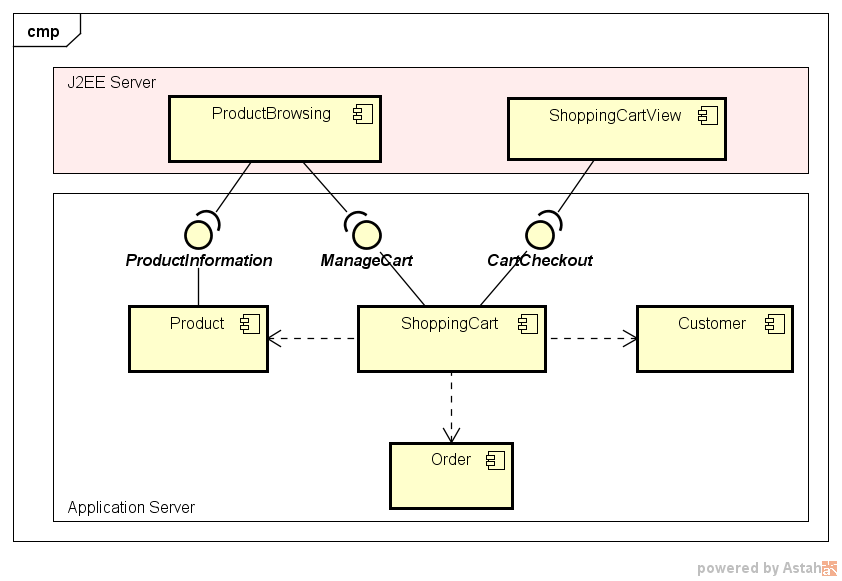
\includegraphics[trim=40 40 23 50,clip,width=0.73\textwidth]{images/uml/component_diagram.png}
    \caption{Example logical architecture -- browsing for products and purchasing them.}
    \label{fig:componentDiagram}
\end{figure}

As was shown in figure \ref{fig:deploymentDiagram},
the \texttt{ProductBrowsing} and \texttt{ShoppingCartView} components are deployed on the J2EE server.
These two component provide the user interaction behaviour in the web application
of browsing for products, adding them to the shopping cart, and purchasing the products.

The \texttt{Product}, \texttt{ShoppingCart}, \texttt{Order} and \texttt{Customer} components are deployed on the application server.
These components deliver the logical behaviour of providing information about products, tracking what is in the shopping cart, and placing orders.

The \texttt{ProductBrowsing} component uses the \texttt{\textsl{ProductInformation}} and \texttt{\textsl{ManageCart}} interfaces.
These two interfaces are realised (or implemented) by the \texttt{Product} and \texttt{ShoppingCart} components respectively.
The \texttt{ShoppingCartView} component uses the \texttt{\textsl{CartCheckout}} interface, which is realised by the \texttt{ShoppingCart} component.
These interfaces describe the communication pathways between the components on the different nodes of the physical architecture.

The \texttt{ShoppingCart} component uses the \texttt{Product}, \texttt{Customer} and \texttt{Order} components.
At the programming level, there could be interfaces between these components which are not shown in this diagram.

\noindent
The application database is not shown in this component diagram as all of its behaviour is defined within the application server's logic.
JPA automates the process of saving and retrieving objects from a relational database.
Consequently, the database is just a storage mechanism and does not implement any application logic.
If the database implemented logic (e.g. through stored procedures and constraints),
then components representing that logical behaviour would be included in this diagram.

\subsubsection{Component Diagram Notation}\label{sec:componentNotation}
As indicated in \ref{sec:deploymentNotation}, rectangles with the `plug' icon represent \emph{components} in UML.

Circles represent \emph{interfaces}, and are labelled with the interface's name.
A line from a component to an interface circle indicates that the component provides (or realises) the interface.

Cups represent a \emph{required interface}, and a line from a component to a cup indicates that the component depends on (or uses) the interface.
This notation visualises the connection between components.

Dependency arrows point from a component whose runtime behaviour depends on behaviour provided by the target component.

Boxes around groups of components are \emph{subjects}.
They represent a logical grouping of elements in a UML diagram and can be given a name to describe the grouping.
Colours and shading can be used to help distinguish between different logical groups.
In this example, the J2EE Server and Application Server subjects represent system boundaries for the two respective deployment environments.

\subsubsection{Behaviour Structure}\label{sec:behaviourStruct}
For complex systems, describing how important behaviour is implemented can aid in understanding the intent of the architecture's design.
UML sequence and communication diagrams can describe this behavioural structure.
Figure \ref{fig:sequenceDiagram} is a high-level sequence diagram describing how the
\texttt{ProductBrowsing} component in the J2EE server collaborates with the
\texttt{ShoppingCart} component on the application server to enable a customer to add a product to their shopping cart.
It also shows the \texttt{ShoppingCart} component communicating with the application database.

\begin{figure}[h!]
    \centering
    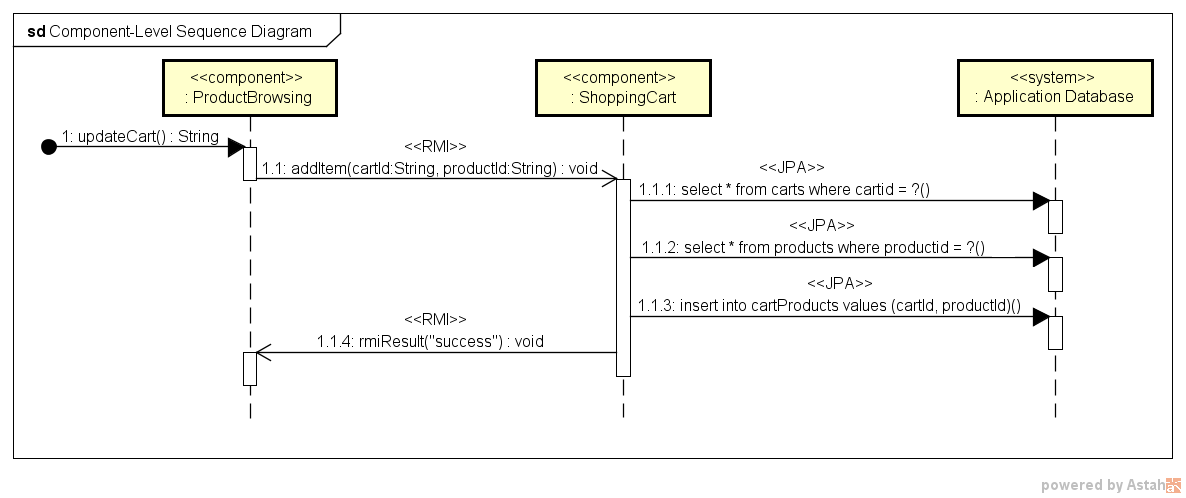
\includegraphics[trim=28 75 23 44,clip,width=\textwidth]{images/uml/component-level_sequence_diagram.png}
    \caption{Example behavioural description -- customer adding a product to their shopping cart.}
    \label{fig:sequenceDiagram}
\end{figure}

Figure \ref{fig:sequenceDiagram} does not provide much additional information that is not already shown or implied by
figures \ref{fig:deploymentDiagram} and \ref{fig:componentDiagram}.
Normally sequence or communication diagrams are used to describe behaviour that is not clear from other diagrams and descriptions.
This can include complex interactions between modules, complex concurrency, real-time constraints, or latency constraints.

\noindent
For example, when Boeing was upgrading the combat control system of the \link{F-111}{https://www.youtube.com/watch?v=xUcpZJE050s}
for the Australian Airforce, they designed a software architecture that used
\link{CORBA}{https://www.ibm.com/docs/en/integration-bus/9.0.0?topic=corba-common-object-request-broker-architecture} as middleware.
The implementation of the middleware caused a fixed delay in sending messages between components.
From an architectural design perspective, it was important to document this delay and enforce a maximum delay on the time taken to complete any process.
A sequence diagram can use constraints to indicate these types of real-time restrictions in your design.

\subsubsection{Sequence Diagram Notation}\label{sec:sequenceNotation}
Sequence diagrams are read from the top down.
The top of the diagram represents the start of the scenario, and execution time progresses down the diagram.
The bottom of the diagram is the end of the scenario.
Duration constraints can be placed between messages indicating information like the maximum allowed time between the start and end of a message.

Rectangles with lines descending from them are \emph{lifelines}.
They represent an instance of a participant in the scenario being described.
The name at the top of a lifeline describes the participant.
In figure \ref{fig:sequenceDiagram}, these are components or the database system.

The horizontal lines are \emph{messages} sent between participants.
Messages use hierarchical numbers to indicate both nesting and sequence of messages.
Message 1.1 is sent by message 1. Message 1.1.1 comes before message 1.1.2.
Message 1 in figure \ref{fig:sequenceDiagram} is a \emph{found message}, meaning that the sender of the message is not shown in the diagram.

A closed arrowhead on a message (e.g. message 1) indicates that it is a synchronous message.
An open arrowhead on a message (e.g. message 1.1) indicates that it is an asynchronous message.
In figure \ref{fig:sequenceDiagram}, stereotypes have been placed on most messages to indicate the protocol used to send the message.

The vertical rectangles sitting on top of lifelines are \emph{execution specifications}.
They indicate when an instance is executing logic.
For example, after the asynchronous message 1.1 is sent to the \texttt{ShoppingCart} component,
message 1 finishes executing.
When the synchronous message 1.1.1 is sent to the database, message 1.1 is still active
as it is waiting for message 1.1.1 to finish before message 1.1 can continue to the next part of the logic.

\subsection{Module View}\label{sec_moduleView}
Figure \ref{fig:classDiagram} uses a UML class diagram as a visual representation of the static structure
of the classes that implement the \texttt{ShoppingCart} component as part of the module view.
Usually only architecturally significant operations and attributes are shown.
(e.g. Operations and attributes needed to understand relationships and behaviour in the component-and-connector view.)
And for simplicity in this diagram, only the classes and interfaces related to adding items to a shopping cart and checking out are shown.

\begin{figure}[h]
    \centering
    \begin{adjustwidth}{-10.5mm}{-11mm}
        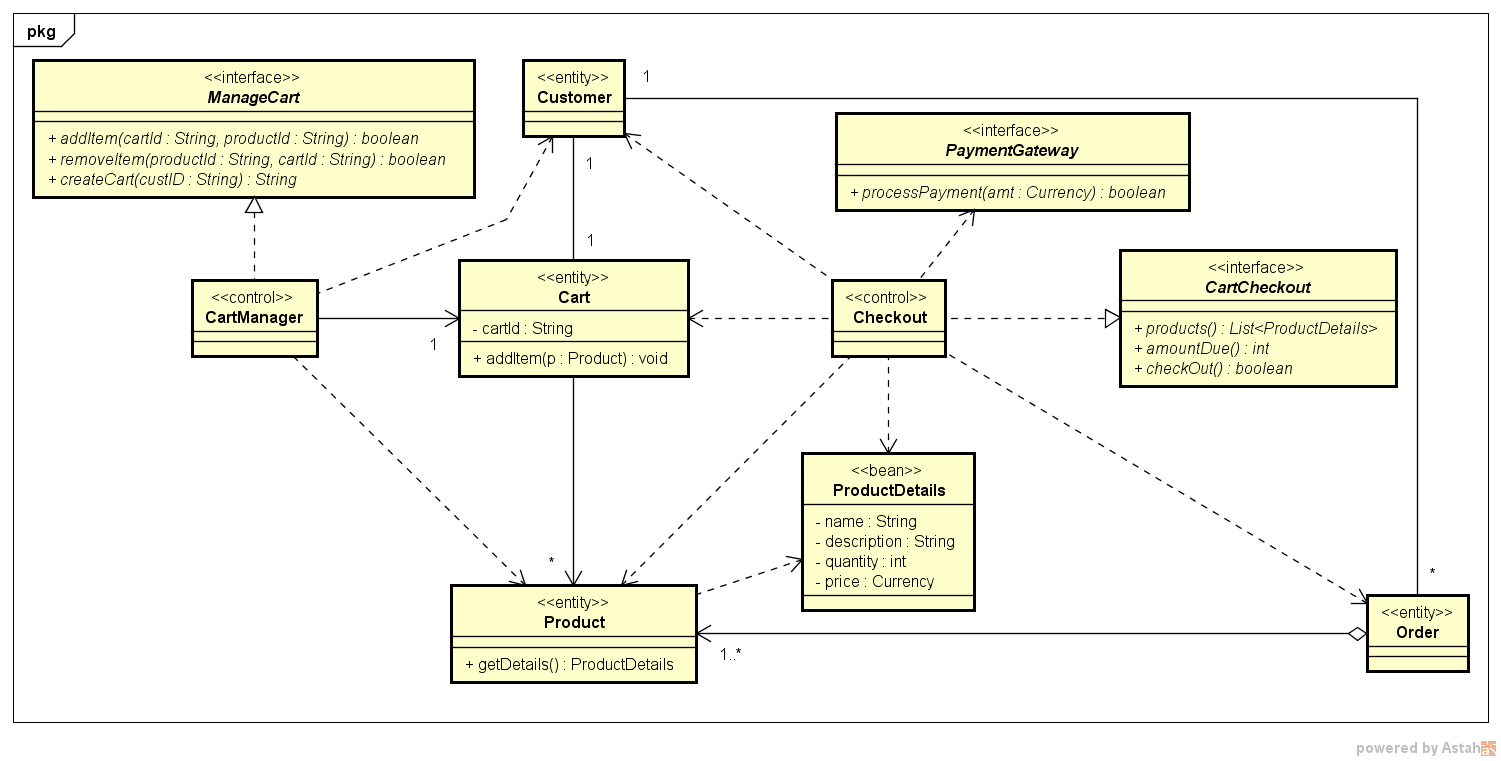
\includegraphics[trim=22 45 22 44,clip,width=0.98\paperwidth]{images/uml/shopping_cart_class_diagram.png}
    \end{adjustwidth}
    \caption{Example static structure for part of the shopping cart package in the class model.}
    \label{fig:classDiagram}
\end{figure}

\noindent
The \texttt{CartManager} and \texttt{Checkout} control classes implement, respectively,
the \texttt{\textsl{ManageCart}} and \texttt{\textsl{Cart\-Check\-out}} interfaces.
These two classes implement the Façade design pattern and manage how
adding products to a shopping cart and checking out are delivered by the classes in this package.
Going back to the component and connector view (figure \ref{fig:componentDiagram}),
when a customer, via their web browser, selects to add a product to their shopping cart,
the \texttt{ProductBrowsing} component's logic uses the \texttt{\textsl{ManageCart}}
interface's \texttt{additem} operation to send a message to the \texttt{ShoppingCart} component.

In the implementation of the \texttt{ShoppingCart} component,
the \texttt{CartManager} class uses the cart and product JPA data access objects (DAOs)
to load the product details and the customer's shopping cart from the application database.
The DAOs create \texttt{Product} and \texttt{Cart} entity objects, and \texttt{CartManager} adds the product to the cart.
Once this is done the \texttt{CartDAO} is used to save the updated cart data into the database.

When a customer wants to checkout the products in their shopping cart, the \texttt{ShoppingCartView} component
uses the \texttt{\textsl{Checkout}} interface's \texttt{products} operation to get a list of the product details to be displayed in the shopping cart.
The \texttt{ProductDetails} class is a Java bean that is used to pass the data about each product to the \texttt{ShoppingCartView}.
Once a customer decides to buy the products in their shopping cart,
the \texttt{ShoppingCartView} sends the \texttt{checkOut} message to the \texttt{ShoppingCart}.
\texttt{Checkout} uses the \texttt{\textsl{PaymentGateway}} interface to process the payment.

\subsubsection{Class Diagram Notation}\label{sec:classNotation}
Formally in UML, rectangles represent \emph{classifiers}. A \emph{class} is one type of classifier.
In a class diagram, a rectangle represents a class, unless a keyword is used to indicate that it is a different type of classifier.
Classifier rectangles have three compartments.
The top compartment contains its name and optionally includes a keyword, stereotypes and properties for the classifier.
The middle compartment contains \emph{attributes}.
The bottom compartment contains \emph{operations}.

Solid lines represent \emph{associations}, which may optionally have an arrow indicating the direction of the relationship.
An association indicates a structural relationship between classes.
Typically this means that the target of an association will be an implicit attribute of the class.
The end of an association can use \emph{multiplicity} to indicate the number of objects of the class that may take part in the relationship.

\noindent
A diamond on the end of an association indicates \emph{aggregate} relationship.
The diamond is on the end that is the aggregate, and the other end is the part.
The diamond may be filled or not. A filled diamond represents \emph{composition} in UML.
This indicates `ownership', where the aggregate controls the lifespan of the part.
A hollow diamond, as in the relationship between \texttt{Order} and \texttt{Product},
indicates \emph{aggregation} in UML.
This is a weaker relationship than composition, as the aggregate does not control the lifespan of the part,
but it still indicates a strong relationship between the classes.

A dashed line with an open arrowhead (e.g. from \texttt{CartManager} to \texttt{Product})
indicates that one classifier \emph{depends} on (or uses) another. This is meant to indicate a transient relationship.

A dashed lines with a closed and hollow arrowhead (e.g. from \texttt{Checkout} to \texttt{\textsl{CartCheckout}})
indicates that the class is \emph{realising} (or implementing) that interface.

\textit{Italicised} names indicate an abstract classifier. Keywords are used to indicate the type of a classifier.
In this example, the keyword \guillemotleft interface\guillemotright~indicates that the classifier is an interface.
Stereotypes use the same notation as keywords. Three standard stereotypes for classes in UML are:
\begin{description}[nosep,left=5mm]
    \item[\guillemotleft entity\guillemotright] Represents a concept (\emph{entity}) from the problem domain.
    \item[\guillemotleft control\guillemotright] Provides logical behaviour from the solution domain.
    \item[\guillemotleft boundary\guillemotright] Communicates with something outside of the system. (Not shown in diagram.)
\end{description}
An additional stereotype \guillemotleft bean\guillemotright~is used to indicate that the class is a Java bean.

\subsubsection{Detailed Behaviour Structure}\label{sec:detailedBehaviourStruct}
Figure \ref{fig:detailedSequenceDiagram} is a detailed sequence showing how the class model in
figure \ref{fig:classDiagram} implements the behaviour of a customer adding a product to their shopping cart.
Like with the high-level sequence diagram, you would only provide detailed sequence diagrams to describe architecturally important details of the design.

\begin{figure}[h!]
    \centering
    \begin{adjustwidth}{-11mm}{-11mm}
        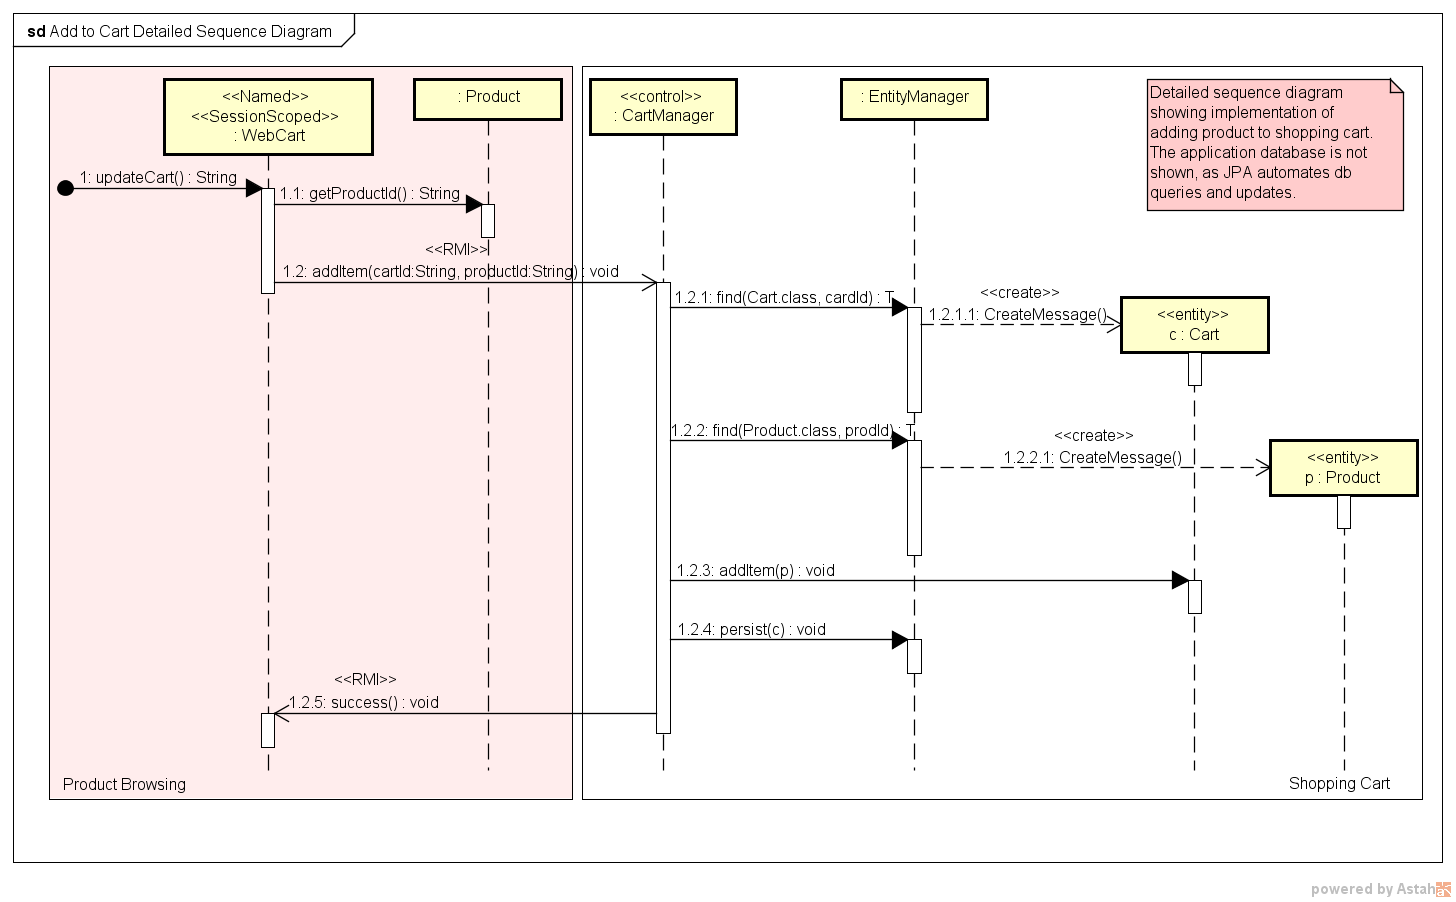
\includegraphics[trim=35 70 31 49,clip,width=0.98\paperwidth]{images/uml/detailed_sequence_diagram.png}
    \end{adjustwidth}
    \caption{Example detailed sequence diagram showing the implementation of customer adding a product to their shopping cart.}
    \label{fig:detailedSequenceDiagram}
\end{figure}

\noindent
The scenario starts with the JSF session-scoped bean \texttt{WebCart} receiving the \texttt{updateCart} message from the browser.
\texttt{WebCart} retrieves the product id and uses the \texttt{ManageCart} interface to send it, along with the cart id,
to the \texttt{ShoppingCart} component on the application server.
The \texttt{ManageCart} interface is implemented by the \texttt{CartManager} class in the \texttt{ShoppingCart} component.

The \texttt{CartManager} uses two JPA data access objects (DAOs) to retrieve the cart and product entities from the application database.
Once the product is added to the cart, the \texttt{CartDAO} saves the updated cart details to the database.
Upon successfully saving the updated cart, the \texttt{CartManager} notifies the \texttt{WebCart}
object in the \texttt{ProductBrowsing} component in the J2EE server.

\subsubsection{Sequence Diagram Notation}
The \guillemotleft create\guillemotright~and \guillemotleft destroy\guillemotright~stereotypes indicate when instances are created or destroyed.
When an instance is created, its lifeline starts at the level of the sequence diagram that indicates the time when it is created.
When an instance is destroyed, its lifeline finishes, with a large \texttt{X}.
Lifelines that are at the top of the diagram indicate instances that existed before the start of the scenario.
Lifelines that reach the bottom of the diagram indicate instances that still exist after the end of the scenario.

In figure \ref{fig:detailedSequenceDiagram}, system boundary boxes are used to indicate which objects execute on which nodes from the deployment diagram.